\documentclass[11pt]{article}
\usepackage{graphics,epsfig,amsmath,amssymb}
\usepackage{epsf}
\usepackage{boxedminipage}
\usepackage{fullpage}
\usepackage{fancyheadings}
\usepackage{times}
\usepackage{amsmath}
\usepackage{ifthen}
%\usepackage{pseudocode}
\usepackage{psfrag}
\pagestyle{fancy}

\setlength{\topmargin}{.2in}
\setlength{\parindent}{0in}
\setlength{\parskip}{.15in}
\setlength{\footskip}{0.1in}

\newcounter{pctr}
\stepcounter{pctr}

\newcounter{partctr}

\newcommand{\ie}{{\em i.e.}}
\newcommand{\eg}{{\em e.g.}}

\newcommand{\ch}{\item {\bf True~~/~~False~~}}
\newcommand{\tfnote}{\probnote{Circle True or False for each choice.}}
\newcommand{\allapply}{\probnote{Circle ALL that apply}}
\newcommand{\bestanswer}{\probnote{Circle the BEST answer}}
\newcommand{\ansbelow}{\probnote{Answer legibly in the space below.}}

\renewcommand{\thesection}{{\bf\Roman{section}}}
\renewcommand{\theenumi}{{\bf\Alph{enumi}.}}
\renewcommand{\labelenumi}{{\bf\Alph{enumi}.}}

\newcommand{\setversion}[1]{\def\version{#1}}
\setversion{answers}
%\setversion{quiz}

\ifthenelse{\equal{\version}{answers}}{
    \newcommand{\sols}[1]{#1}
}{
    \newcommand{\sols}[1]{}
}


\newcounter{answer}
\newenvironment{answer}[1][\relax]{\refstepcounter{answer}\begin{list}%
 {}{\leftmargin 0pt\rightmargin 0pt\labelsep 3pt\parsep 0pt%
 \setlength{\listparindent}{\parindent}}
    \item {\bf Answer \theanswer #1}\
    }{\hspace*{\fill}$\blacksquare$\end{list}} 



% uses these macros to delimit problems
\newcommand\prob[1]%
  {\begin{itemize}\item[]%
   \vspace{.2in}{\bf\thepctr. ~[#1~ points]:}\stepcounter{pctr}}
\newcommand\eprob{\end{itemize}}
\newcommand\probnote[1]%
  {\\\begin{tabular}{cr} \hspace{3in} & {\bf (#1)} \\ \end{tabular}}

% headers/footers
\lhead[\fancyplain{}{\bf Page \thepage ~of \pageref{lastpage}}]%
      {CS 6250 Fall 2010, Practice Quiz}
\lfoot[{\bf Initials: }]%
      {{\bf Initials: }}
\rhead[CS 6250 Spring 2008, Quiz 1]%
      {\fancyplain{}{\bf Page \thepage ~of \pageref{lastpage}}}
\cfoot{}
\setlength{\headrulewidth}{0in}
\setlength{\headsep}{.3in}

 % Compact itemize and enumerate.  Note that they use the same counters and
% symbols as the usual itemize and enumerate environments.
\def\compactify{\itemsep=0pt \topsep=0pt \partopsep=0pt \parsep=0pt}
\let\latexusecounter=\usecounter
\newenvironment{CompactItemize}
  {\def\usecounter{\compactify\latexusecounter}
   \begin{itemize}}
  {\end{itemize}\let\usecounter=\latexusecounter}
\newenvironment{CompactEnumerate}
  {\def\usecounter{\compactify\latexusecounter}
   \begin{enumerate}}
  {\end{enumerate}\let\usecounter=\latexusecounter}

\begin{document}
\cfoot{}
\pagestyle{empty}
\begin{center}
\begin{tabular}{lr}
\resizebox{1in}{!}{
\includegraphics{GT}}
&
\parbox{4in}{
    {\Large\it College of Computing} \\ \\
    {\LARGE\sf Georgia Institute of Technology} 
}
%
\end{tabular}
\end{center}

\begin{center}
{\Large{\bf CS 6250: Computer Networking: Fall 2010} \\
 \vspace{.15in} \Huge{\bf Practice Quiz}} 
\vspace{.2in}

% this is the box on the first page with overall quiz information
\begin{boxedminipage}[h]{6in}
There are \underline{XXX questions} and
  \underline{\pageref{lastpage} pages} in this quiz booklet (including
  this page).  Answer each question according to the instructions given.
  You have {\bf 85 minutes} to answer the questions.

%\vspace{.1in} The last page is an easy question.  {\em Rip this
%page off of your exam for five bonus points.}  Turn it in anonymously if
%you like.


\vspace{.1in} 
If you find a question ambiguous, write down any
assumptions you make.  {\bf Be neat and legible.}  If I can't
understand your answer, I can't give you credit!  There are three pretty
challenging questions (clearly marked); you may want to look through the
whole quiz and save those for last.

\vspace{.1in} 
Use the empty sides of this booklet if you need scratch space.  You
may also use them for answers, although you shouldn't need to.  {\em If you
do use the blank sides for answers, make sure to clearly say so!}

\vspace{.1in} 
{\bf Note well: Write your name in the space below AND your initials at the bottom of each
page of this booklet.}

\begin{center}{\bf THIS IS AN ``OPEN NOTES, OPEN PAPERS'' QUIZ.\\
NO OTHER MATERIALS, NO PHONES, NO COMPUTERS, NO LAPTOPS, NO PDAS.\\
NO ENCRYPTED WIRELESS TRAFFIC. \\
MAKE SURE YOU'VE READ ALL THE INSTRUCTIONS ABOVE!}
\end{center}
{\em Initial here to indicate that (1)~you've read the instructions and (2)~
you agree to abide by the Georgia Tech Honor Code: }



\vspace{.1in} The last page has easy bonus questions, which you can
answer outside of the allotted time.  Rip the last page off of your
quiz for five bonus points.  Turn it in anonymously if you like.

\end{boxedminipage}
\end{center}
\vspace*{0.25in}
\begin{center}
{\it Do not write in the boxes below}
\end{center}

\begin{center}
\begin{tabular}{|l|l|l|l|l|l|l|l|l|} \hline \hline
{\bf XX-XX (xx/XX)}& {\bf XX-XX (xx/XX)}& {\bf 11-14 (xx/XX)} &{\bf Bonus (xx/5)} & {\bf Total
  (xx/XX)}  \\ \hline 
 & & & & \\ 
 & & & &\\ \hline \hline
\end{tabular}
\end{center}

\vspace{.2in}
{\bf\Large{Name:}}

\newpage
\pagestyle{fancy}

\section{Warmup}

\prob{4} Which of the following is true about Address Resolution
Protocol (ARP) and learning bridges?
\allapply

\setcounter{partctr}{0}
\begin{list}{\bf\Alph{partctr}.}{\usecounter{partctr}}
\item A learning bridge maintains state that maps IP addresses to hardware
  (MAC) addresses.
\item A learning bridge maintains state that maps IP addresses to MAC
  addresses. 
\item A host's ARP table maintains state that maps IP addresses to hardware
  (MAC) addresses.
\item A host's ARP table maintains state that maps hardware addresses to IP
  addresses. 
\end{list}
\eprob

\sols{
\begin{answer}
The answer is: (A), (C).
\end{answer}
}


\prob{4} Which of the following is true about DNS?
\allapply
\setcounter{partctr}{0}
\begin{list}{\bf\Alph{partctr}.}{\usecounter{partctr}}
%\begin{enumerate}
\item A query for an {\tt A} record may return multiple IP addresses in
  the response.
\item A query for an {\tt NS} record may return multiple IP addresses in
  the response.
\item A query for a {\tt MX} record may return multiple IP addresses in
  the response.
\item A short TTL on an {\tt A} record reply may run the risk of
  increasing traffic at the root nameserver.
\item None of the above.
\end{list}
\eprob

\sols{
\begin{answer}
The answer is: (A), (C).
\end{answer}
}

\pagebreak
\prob{2} Which of the following most accurately describes the {\em most common}
uses for eBGP, iBGP, and IGP?
\bestanswer
\setcounter{partctr}{0}
\begin{list}{\bf\Alph{partctr}.}{\usecounter{partctr}}
%\begin{enumerate}
\item eBGP is used between ASes for external destinations, iBGP is used
  within an AS for external destinations, and IGP is used within an AS
  for destinations within an AS.
\item eBGP is used
  within an AS for external destinations, iBGP is used between ASes for
  external destinations, and IGP is used within an AS for internal destinations.
\item eBGP is used between ASes for external destinations, iBGP is used
  within an AS for internal destinations, and IGP is used within an AS
  for external destinations.
\item None of the above
\end{list}
\eprob

\sols{
\begin{answer}
The answer is (A).
\end{answer}
}


\prob{4} Which of the following might the operator of an AS use for {\em
  inbound} traffic engineering (i.e., to control how traffic reaches the
  destinations in its network)?
\bestanswer
\setcounter{partctr}{0}
\begin{list}{\bf\Alph{partctr}.}{\usecounter{partctr}}
%\begin{enumerate}
\item AS path prepending
\item Selectively advertising prefixes on some BGP sessions but not
  others
\item Adjusting local preference settings for routes learned from
  neighboring ASes
\item None of the above
\end{list}
\eprob

\sols{
\begin{answer}
The answer is (A), (B).
\end{answer}
}

\prob{4} Suppose that a link is being monitored with both packet flow
monitoring and a full packet trace.

Assume that routes do not change, the interface and packet filters do
not drop any packets, that the packet trace contains full payloads, and
that the flow records are based on {\em all} packets that traverse the
link (\ie, that there is no sampling).

Which of the follow statements are true about each of the traces?  
\allapply

\setcounter{partctr}{0}
\begin{list}{\bf\Alph{partctr}.}{\usecounter{partctr}}
%\begin{enumerate}
\item The packet trace can be used to calculate the exact duration of
  every flow that crosses the link.
\item The trace of flow records can always be used to calculate the
  exact duration of every flow that crosses the link.
\item Both the packet trace and the trace of flow records can be used to
  determine the number of bytes in each flow.
\item The size of a flow record will always be smaller than
  the combined size of the packets in the corresponding flow.
\end{list}
\eprob

\sols{
\begin{answer}
The answer is (A) and (C).  (B) is false because a single
flow may be split across multiple flow records, so it may be tough to
distinguish when a flow begins and ends if it is idle for a long time.
(D) is false; recall the example in class where we discussed that a
single flow could consist of a SYN packet, while a typical flow record
is 1500 bytes.
\end{answer}
}



\newpage
\section{Potpourri}

\prob{4} Recall that in class we discussed that the Georgia Tech network
has hundreds of virtual LANs.  State {\em two advantages} for dividing a
single network into multiple VLANs.~\ansbelow
\vspace{1.25in}
\eprob

\sols{
\vspace{-1.25in}
\begin{answer}
Multiple VLANs divide the network into smaller broadcast domains, which
can provide various improvements for, say, security (it's much harder to
``snoop'' traffic on a different LAN) and scaling (reducing the size of
each broadcast domain allows the network to scale better).
\end{answer}
}


\pagebreak
\prob{2} Recall from Hands-On Assignment 1, the Click {\tt FromHost}
module for your Ethernet switch had to be set in promiscuous mode.
Explain why the switch would not forward Ethernet frames if this was not
the case.  ~\ansbelow
\vspace{1.25in}
\eprob

\sols{
\vspace{-1.25in}
\begin{answer}
In this assignment, the {\tt EtherSwitch} needed to be set in
promiscuous mode because ethernet frames from a nost connected to the
switch would have a destination MAC address for the host to which the
frame was destined.  However, the {\tt EtherSwitch} in the Emulab
testbed is simply another host with interfaces: if the interface on that
nodes is not set to promiscuous mode, it will not accept a frame that
does not have a MAC address that corresponds to the MAC address of its
own interface.
\end{answer}
}



\pagebreak
\prob{4} Consider the graph below, which shows a cumulative distribution
function (CDF) of the DNS response times for DNS lookup latencies for
three data traces: (1)~two different traces at a resolver at MIT in
Cambridge, MA; (2)~one trace at a resolver in Korea ({\tt
  kaist}).~\footnote{In case you don't know, the way to read a CDF is as
  follows: a point $(x,y)$ means that for that distribution, the
  fraction $y$ of the points in that distribution have value $x$ or
  smaller.  For example, slightly more than 30\% of the queries in the
  {\tt kaist} trace had a lookup latency of 10ms or less.}
\setcounter{partctr}{0}
\begin{list}{\bf\Alph{partctr}.}{\usecounter{partctr}}
\item Which resolver has more queries that take more than a second to
  resolve? 
\item Why might the two traces have different latency distributions?
  (In other words, why might one resolver take longer to resolve queries
  than another?)  There are several possible reasons; give one.  ({\em
    Hint:} Think about geography.)
\end{list}
~\ansbelow 
\begin{center}
\resizebox{0.45\textwidth}{!}{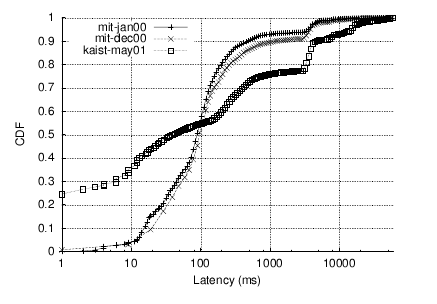
\includegraphics{dns}}
\end{center}
\vspace{2in}
\eprob


\sols{
\vspace{-1in}
\begin{answer}
Korea (kaist) has more queries that take more than a second to resolve.
The two traces likely have different latency distributions because the
local resolvers are located in different geographic regions, but the
lookup distributions themselves may also vary.  For example, it is
likely that a local resolver in Korea will have more DNS queries for
authoritative domains that are within Korea than one in the US, but also
a local resolver in Korea will likely have a significantly larger number
of queries that are for domains that are very far away (i.e., in the US).
\end{answer}
}

\newpage
\section{Design Question: Scaling Ethernet}

Recall the Ethernet switch topology from Hands-On Assignment~1, shown
below.  You installed learning bridges on a dumbbell topology.  Learning
bridges can control some flooding of data traffic, but 1other broadcast
traffic (e.g., ARP queries, DHCP) will still be flooded across the
entire LAN.


\prob{2} Explain why flooding ARP queries across the entire network
could impose scaling problems.
~\ansbelow
\vspace{1.25in}
\eprob

\sols{
\vspace{-1in}
\begin{answer}
Flooding ARP queries across the entire network could impose scaling
problems by introducing a substantial amount of broadcast network
traffic, unnecessarily wasting network capacity.  
\end{answer}
}

George Burdell has an idea about how to make Ethernet scale by cutting
down ARP traffic: ``Instead of flooding ARP queries to all nodes on the
LAN, why not simply have an ARP directory server?''  He suggests that a
single machine on a LAN could maintain a table of IP-to-MAC address
mappings.

\prob{4} Explain the advantages of making the ARP directory server state
``soft''. 
~\ansbelow
\vspace{1.25in}
\eprob

\sols{
\vspace{-1in}
\begin{answer}
In this case, soft state provides benefits for both host mobility and
for resilience.  If the ARP directory server state is soft, then the
directory server can maintain mappings between IP address and MAC
address, even as hosts move or even if the directory server crashes.
\end{answer}
}

\newpage
Georgia Tech takes George's suggestion and deploys the ARP directory
server, but the operators noticed that the server is sustaining heavy
query loads during peak hours.  They decide that they would like to {\em
distribute} the ARP directory and see two possibilities for distributing
the service:
\begin{enumerate}
\itemsep=-1pt
\item Each directory server maintains a complete copy of
  the ARP table.  Any server can answer an ARP query for any IP address
  on the LAN.
\item Each directory server maintains only a {\em subset} of the ARP
  table.  In other words, each directory server can resolve queries for
  some MAC addresses. {\em The ARP query must be ``routed'' to the
    correct directory server.}
\end{enumerate}

\prob{4} 
Give one advantage and one disadvantage of each approach.  (Hint:
Think about issues such as how well each approach scales, traffic load,
potential consistency issues, how the table(s) will be populated, etc.)
~\ansbelow
\vspace{1.25in}
\eprob

\sols{
\vspace{-1in}
\begin{answer}
If each directory maintains a copy of the ARP table, then any server can
answer any ARP query.  This simplifies routing of the queries (i.e.,
determining which server can answer which query), and it also makes the
system robust if any one of the ARP directory servers crashes.  However,
it potentially makes the system less scalable (since each server must
store all of these mappings), and it makes maintaining consistency more
complicated: when an ARP entry becomes stale or changes (e.g., due to
host mobility), {\em all} of the directory servers must be updated.
\end{answer}
}

After some consideration, the Georgia Tech operators decide to implement
the second option.  

\prob{6} Explain how you might (1)~decide to divide the ARP table among
the directory servers; (2)~establish connectivity between the ARP
directory servers to properly ``route'' the query to the right server,
without flooding. {\em No single ``right'' answer!  Be creative.
  Partial credit will be given for sensible approaches.}  ~\ansbelow
\vspace{1.25in}
\eprob



\newpage
\section{Bonus: Anonymous Course Feedback}

{\bf This page is anonymous.}  Rip this off from your exam, and turn it
in separately if you like.  You'll get five points for simply ripping
off the last page of the exam, but I'd prefer if you fill it out and
hand it in in a separate stack.
\vspace{.5in}

What are the things you like most about the course so far?  Anything is
fair game here (topics, course structure, board technique, etc.).
\vspace{1.5in}


What are the things you like least about the course so far?  Again,
anything is fair game.
\vspace{1in}


What topics would you like to see covered?
\vspace{1in}



\label{lastpage}
\end{document}
